\section{Results}


\begin{frame}{ECG simulator in 32-bit software vs. 8-bit DAC hardware}
\begin{minipage}[c][0.5\textheight][c]{\linewidth}
\begin{center}
    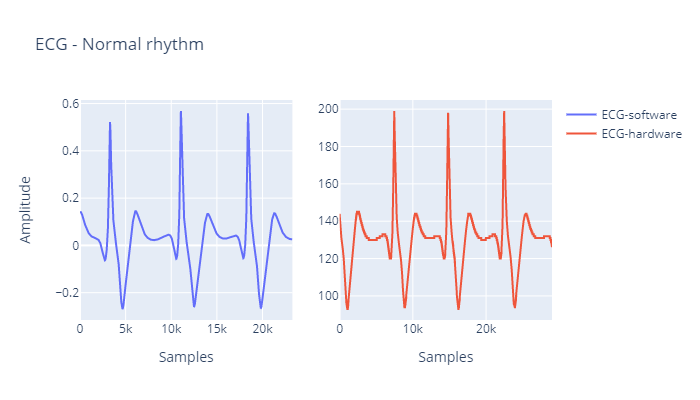
\includegraphics[height=0.8\textheight]{images/Simulator/simulator1.png}  
\end{center}
\end{minipage}
\end{frame}

\begin{frame}{ECG simulator for multiples pathology configurations}
\begin{minipage}[c][0.5\textheight][c]{\linewidth}
\begin{center}
    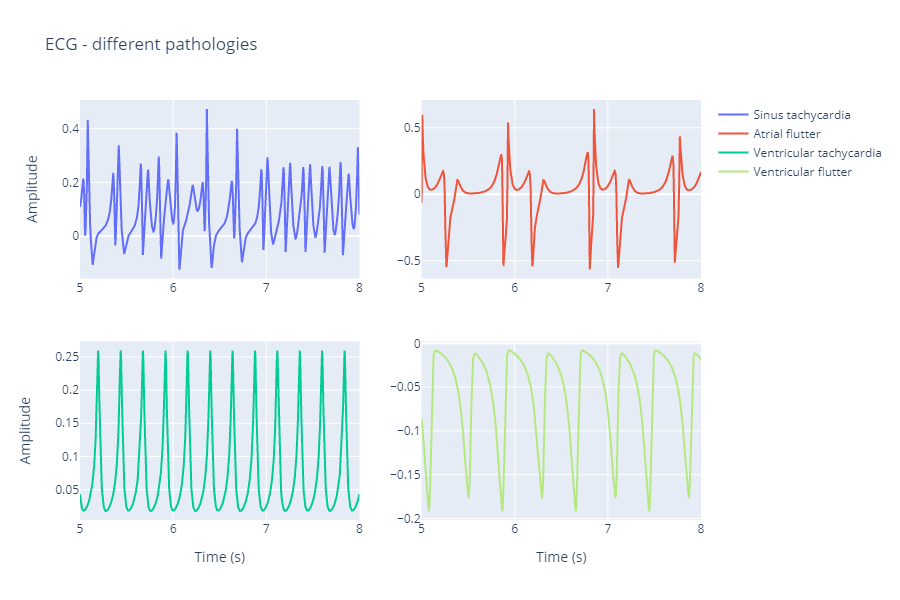
\includegraphics[height=0.8\textheight]{images/Simulator/simulator2.png}  
\end{center}
\end{minipage}
\end{frame}


\begin{frame}{Analog front-end nodes in time domain}
\begin{minipage}[c][0.5\textheight][c]{\linewidth}
\begin{center}
    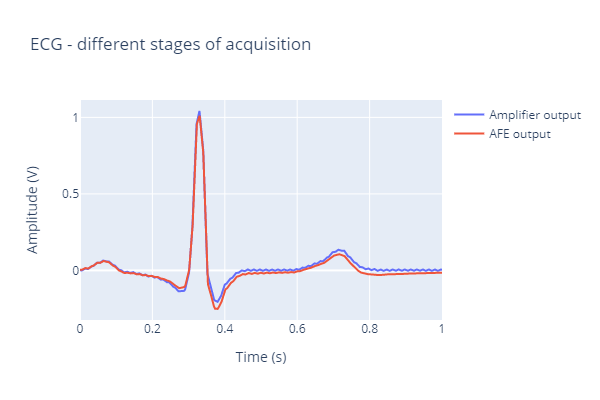
\includegraphics[height=0.8\textheight]{images/AFE/afe2.png}  
\end{center}
\end{minipage}
\end{frame}
\begin{frame}{Analog front-end nodes in frequency domain}
\begin{minipage}[c][0.5\textheight][c]{\linewidth}
\begin{center}
    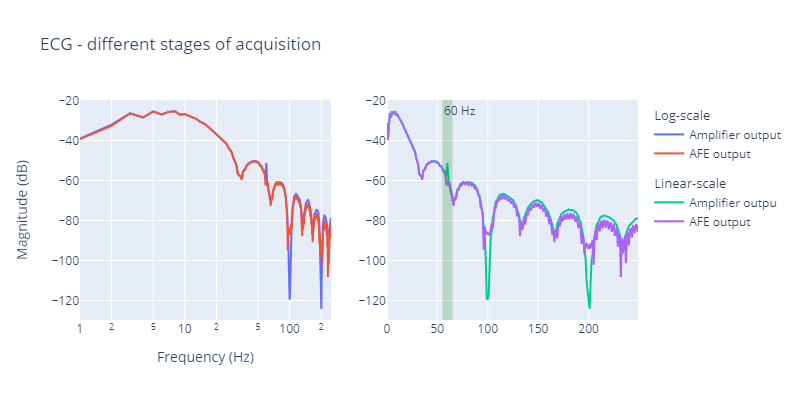
\includegraphics[height=0.8\textheight]{images/AFE/afe4.png}  
\end{center}
\end{minipage}
\end{frame}


\begin{frame}{Heart rate analysis in software}
\begin{minipage}[c][0.5\textheight][c]{\linewidth}
\begin{center}
    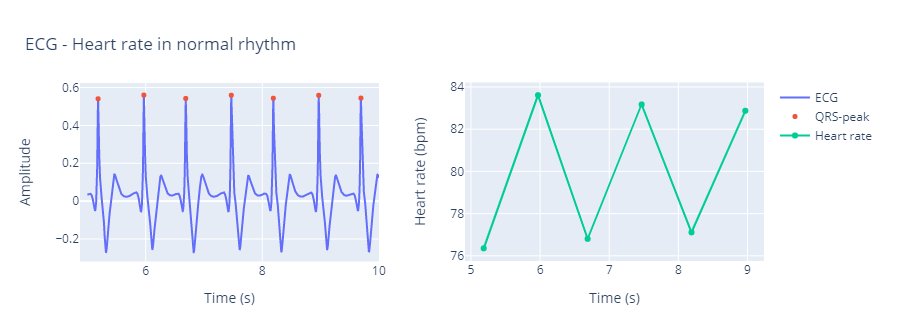
\includegraphics[width=\textwidth]{images/heart_rate/heart_rate_software.png}  
\end{center}
\end{minipage}
\end{frame}

\begin{frame}{Visualization in Python USB client: noisy ECG}
\begin{minipage}[c][0.5\textheight][c]{\linewidth}
\begin{center}
    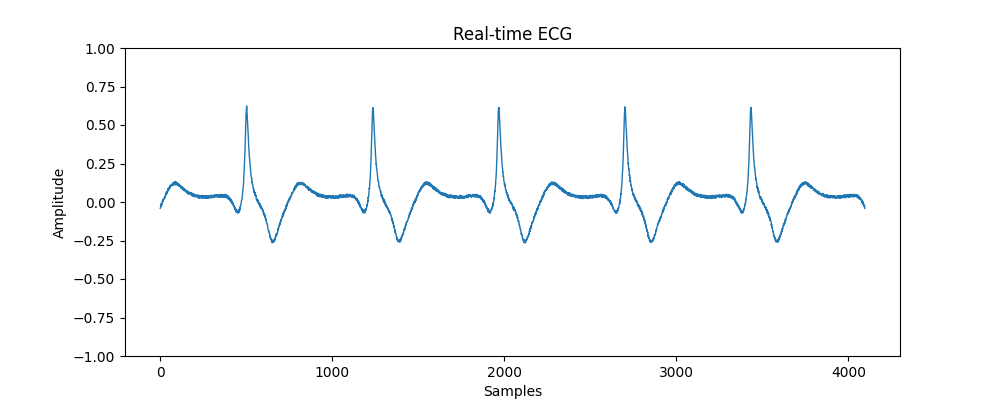
\includegraphics[width=\textwidth]{images/DAQ/daq_ecg_noise.png} 
\end{center}
\end{minipage}
\end{frame}

\begin{frame}{Visualization in Python USB client: filtered ECG}
\begin{minipage}[c][0.5\textheight][c]{\linewidth}
\begin{center}
    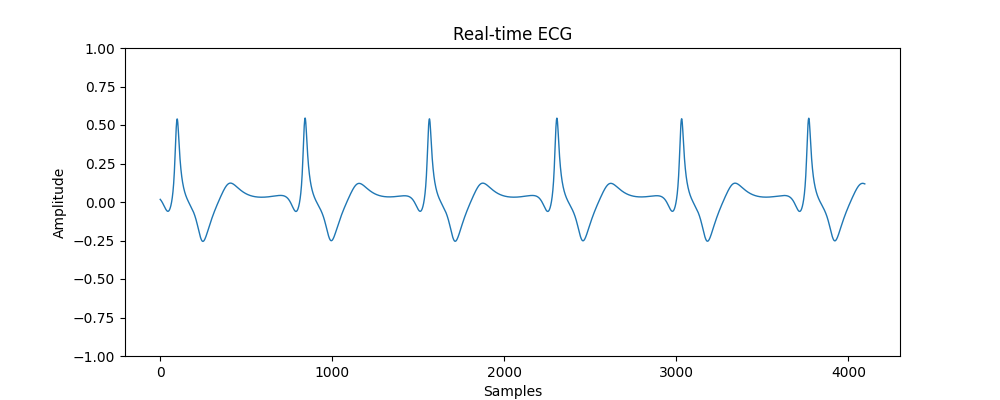
\includegraphics[width=\textwidth]{images/DAQ/daq_ecg_filtered.png} 
\end{center}
\end{minipage}
\end{frame}

\begin{frame}{Visualization in Python USB client: ECG + heart rate}
\begin{minipage}[c][0.5\textheight][c]{\linewidth}
\begin{center}
    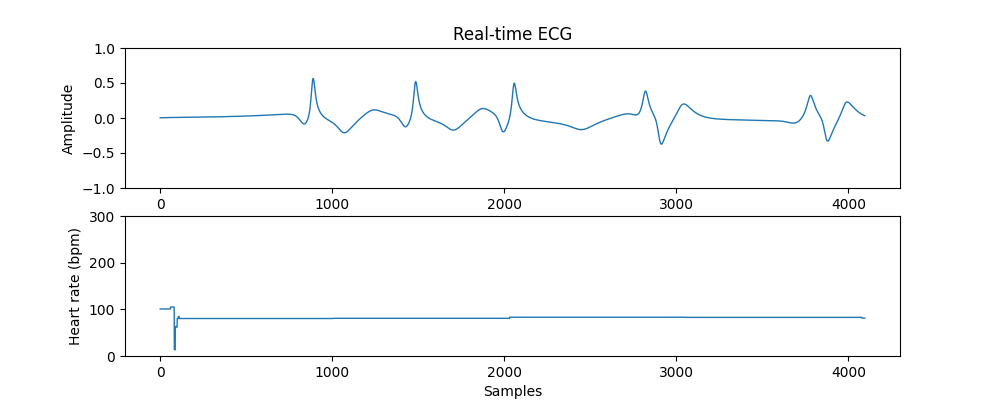
\includegraphics[width=\textwidth]{images/DAQ/daq_heart_rate.png} 
\end{center}
\end{minipage}
\end{frame}
